\chapter{مراحل الحياة}\label{ch:g3:stages-of-life}

انظم صورة عائلية: الرضيع على \omterm{def:g1:my-body:joint}{ركبة} الجدة، والتلميذ الذي فقد سنّين
أماميتين، وابن العم \omterm{def:g3:stages-of-life:stages}{المراهق} الذي صار فجأة أطول من أمه، والوالدان،
والجدة نفسها. أسرة واحدة، وأصيل واحد --- \omterm{def:g2:born-grow-die:cycle}{ودورة حياة} الإنسان كلها
جالسة على أريكة واحدة. وهذه السنة ننظر عن قرب إلى تلك المراحل،
وإلى كيفية قياس النمو نفسه.

\section{مراحل حياة الإنسان}

\begin{definition}[مراحل حياة الإنسان]\label{def:g3:stages-of-life:stages}
تمر حياة الإنسان بمراحل:
\begin{enumerate}
  \item \emph{الرضاعة}\index{رضيع} (السنتان الأوليان تقريبًا):
        أسرع نمو على الإطلاق، وأول الأسنان، وأول الخطوات، وأول
        الكلمات؛
  \item و\emph{الطفولة}\index{طفل}: نمو ثابت، ومقايضة \omterm{prop:g2:teeth-and-eating-well:sets}{الأسنان
        اللبنية} \omterm{prop:g2:teeth-and-eating-well:sets}{بالأسنان الدائمة}، وتعلّم من كل صنف؛
  \item و\emph{المراهقة}\index{مراهق}: دفعة جديدة من النمو
        السريع، وتحول الجسم من جسم طفل إلى جسم بالغ؛
  \item و\emph{البلوغ}\index{بالغ}: انتهاء النمو في الطول؛
        والبالغون يمكن أن يصيروا آباء؛
  \item و\emph{الشيخوخة}\index{شيخوخة}: يبيضّ الشعر، ويتغضّن
        \omterm{def:g1:the-five-senses:sense}{الجلد}، وتتراجع القوة ببطء --- وهي المرحلة الأخيرة
        الطبيعية من الدورة.
\end{enumerate}
\end{definition}

\begin{example}[قراءة الأريكة]\label{ex:g3:stages-of-life:sofa}
على أريكة الأسرة: الرضيع (المرحلة الأولى)، والتلميذ المفلوج
الأسنان (المرحلة الثانية --- وتبديل \cref{ch:g2:teeth-and-eating-well}
في أوجه)، وابن العم في السادسة عشرة (المرحلة الثالثة، في وسط
الدفعة)، والوالدان (المرحلة الرابعة)، والجدة (المرحلة الخامسة).
خمس مراحل، وأسرة واحدة.
\end{example}

\begin{omfigure}
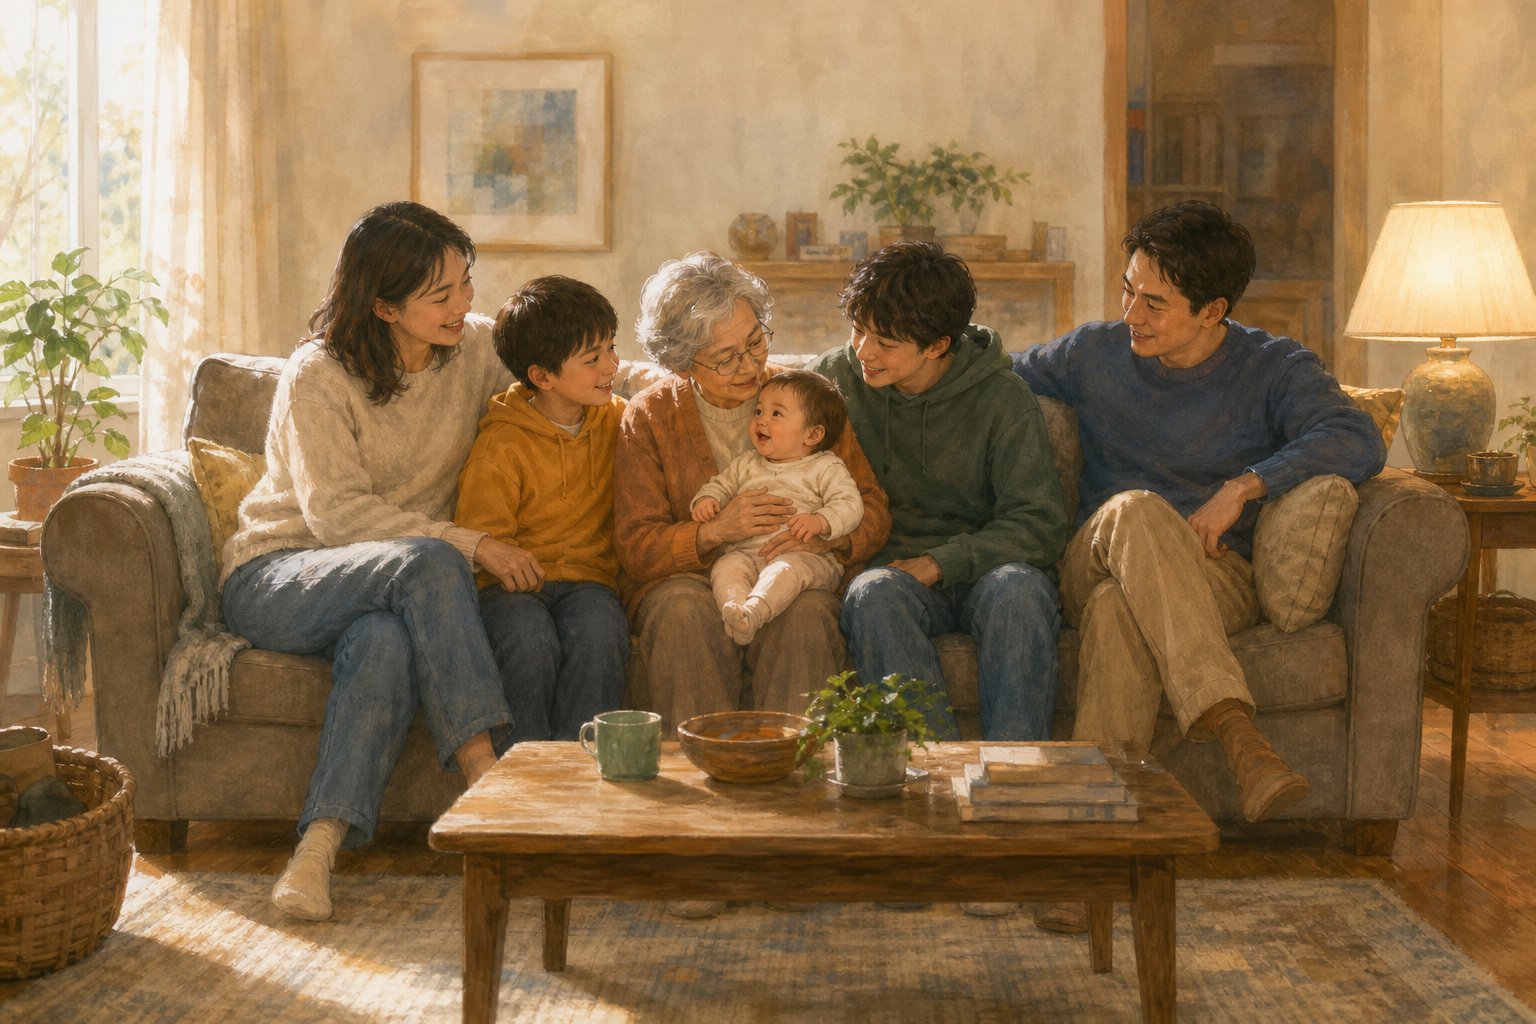
\includegraphics[width=0.62\linewidth]{images/book1/ai/g3-stages-family.png}

{\small الدورة كلها على أريكة واحدة: رضيع، وطفل، \omterm{def:g3:stages-of-life:stages}{ومراهق}، وبالغان،
وجدة.}
\end{omfigure}

\begin{remark}[النمو ليس ثابتًا]\label{rem:g3:stages-of-life:bursts}
للنمو إيقاع: سريع جدًّا عند الرضيع --- إذ يزيد الطول نحو نصفه في
السنة الأولى --- ثم أبطأ وثابت طول \omterm{def:g3:stages-of-life:stages}{الطفولة}، ثم سريع من جديد عند
\omterm{def:g3:stages-of-life:stages}{المراهق}، ثم ينتهي. دفعتان بينهما امتداد هادئ: هذه هي الصورة
الطبيعية للكبر.
\end{remark}

\section{قياس النمو}

\begin{definition}[منحنى النمو]\label{def:g3:stages-of-life:chart}
\emph{منحنى النمو}\index{منحنى النمو} سجل للطول (أو للوزن) يُقاس
مرة بعد مرة عبر الزمن --- وهو علامات إطار الباب في
\cref{ch:g1:my-body}، منتظمة ومؤرخة. ويحتفظ الأطباء بواحد لكل
طفل.
\end{definition}

\begin{omfigure}
\begin{tikzpicture}
\begin{axis}[omaxis,
    width=9.2cm, height=6cm,
    xlabel={العمر (سنة)}, ylabel={الطول (سم)},
    xmin=0, xmax=22.5, ymin=0, ymax=190,
    xtick={0,5,10,15,20},
    ytick={50,100,150},
    ]
  \addplot[very thick, omDef, smooth] coordinates {
    (0,50) (1,75) (2,87) (4,102) (6,115) (8,127) (10,138)
    (12,150) (14,165) (16,175) (18,178) (20,178)
  };
\end{axis}
\end{tikzpicture}

{\small منحنى نمو من \omterm{def:g2:born-grow-die:cycle}{الولادة} إلى \omterm{def:g3:stages-of-life:stages}{البلوغ}: شديد الميل عند الرضيع،
ثابت عند الطفل، شديد الميل من جديد عند \omterm{def:g3:stages-of-life:stages}{المراهق}، ثم مستوٍ ---
فالنمو انتهى.}
\end{omfigure}

\begin{example}[قراءة المنحنى]\label{ex:g3:stages-of-life:reading}
على المنحنى يصعد الخط نحو $\qty{25}{cm}$ في السنة الأولى وحدها ---
ونحو $\qty{6}{cm}$ في السنة فقط طول \omterm{def:g3:stages-of-life:stages}{الطفولة}. والقسمان الشديدا
الميل هما دفعتا \cref{rem:g3:stages-of-life:bursts}؛ أما الطرف
المستوي فيقول إن \omterm{def:g3:stages-of-life:stages}{البالغ} كفّ عن الازدياد طولًا.
\end{example}

\begin{method}[الاحتفاظ بمنحنى نموك]\label{met:g3:stages-of-life:keep}
\begin{enumerate}
  \item قِس الطول بعناية (بطريقة الجدار والكتاب في السنوات
        السابقة)، وبلا حذاء دائمًا؛
  \item واكتب التاريخ والطول في دفتر، أو علّم إطار الباب وأرّخ
        العلامة؛
  \item وأعد القياس كل بضعة أشهر --- فالانتظام أهم من التكرار؛
  \item ولترى الحكاية، ارسم النقاط: العمر على الأسفل، والطول على
        الجانب، كما في الشكل.
\end{enumerate}
\end{method}

\section{وللحيوانات والنباتات مراحل أيضًا}

\begin{proposition}[المراحل في العالم الحي]\label{prop:g3:stages-of-life:animals}
كل \omterm{def:g1:living-or-not:living}{كائن حي} يمر بمراحل نسخته الخاصة من الدورة --- الصغر، \omterm{def:g3:stages-of-life:stages}{والبلوغ}،
\omterm{def:g3:stages-of-life:stages}{والشيخوخة}. وقد تشبه مرحلة الصغر \omterm{def:g3:stages-of-life:stages}{البالغ} (كالهر الصغير والمهر) أو لا
تشبهه في شيء (كالشرغوف \omterm{ex:g2:animals-grow-up:butterfly}{واليرقة} في \cref{ch:g2:animals-grow-up})؛
ومراحل \omterm{def:g1:plants-around-us:plant}{النبات} تجري: \omterm{def:g2:from-seed-to-plant:seed}{بذرة}، فبادرة، \omterm{def:g1:plants-around-us:plant}{فنبات} صغير، \omterm{def:g3:stages-of-life:stages}{فبالغ} مزهر. وما لا
يستطيعه أي منها هو أن يقفز مرحلة أو يجريها إلى الوراء.
\end{proposition}
\admitted

\begin{example}[ما أسرعها وما أبطأها]\label{ex:g3:stages-of-life:speeds}
تختلف السرعات اختلافًا هائلًا. فالذبابة تبلغ في أسابيع؛ والقطة في
سنة تقريبًا؛ والإنسان في نحو عشرين سنة؛ وشجرة البلوط تستغرق عشرات
السنين قبل أول ثمار بلوطها. وبطيئًا كان أم سريعًا، فترتيب المراحل
لا يتغير أبدًا.
\end{example}

\begin{remark}[الشيخوخة مرحلة لا عيب]\label{rem:g3:stages-of-life:oldage}
الشعر الأبيض والتغضّن ليسا مرضًا: بل هما مرحلة الجسم الأخيرة،
طبيعيان كأول أسنان الرضيع. وفي أنواع كثيرة، وفي الأسر البشرية،
يحمل الكبار ما يحتاج إليه الصغار أكثر من غيره --- الخبرة.
\end{remark}

\section{تمارين}

\begin{exercise}[$\star$]\label{exo:g3:stages-of-life:1}
سمِّ مراحل حياة الإنسان الخمس، مرتبةً.
\end{exercise}

\begin{exercise}[$\star$]\label{exo:g3:stages-of-life:2}
في أي مرحلة: (أ) تسقط \omterm{prop:g2:teeth-and-eating-well:sets}{الأسنان اللبنية}؟ (ب) يستطيع المرء أن يصير
أبًا أو أمًّا؟ (ج) يكون النمو أسرع ما يكون في الحياة كلها؟
\end{exercise}

\begin{exercise}[$\star$]\label{exo:g3:stages-of-life:3}
ما دفعتا النمو، وما الذي يقع بينهما؟
\end{exercise}

\begin{exercise}[$\star$]\label{exo:g3:stages-of-life:4}
على \omterm{def:g3:stages-of-life:chart}{منحنى النمو}، كيف تعرف من الخط وحده أن بالغًا كفّ عن النمو؟
\end{exercise}

\begin{exercise}[$\star$]\label{exo:g3:stages-of-life:5}
بالاستعانة بالمنحنى، كم سنتيمترًا يصعد الخط بين سن $6$ وسن $8$
تقريبًا؟ وكم يصعد في السنة الأولى وحدها؟
\end{exercise}

\begin{exercise}[$\star$]\label{exo:g3:stages-of-life:6}
لماذا يجب أن يُقاس الطول بلا حذاء دائمًا، وبالطريقة نفسها في كل
مرة؟ وما الذي قد يفسد لولا ذلك؟
\end{exercise}

\begin{exercise}[$\star$]\label{exo:g3:stages-of-life:7}
اذكر مراحل حياة شجرة البلوط، من الثمرة إلى الشجرة العجوز.
\end{exercise}

\begin{exercise}[$\star$]\label{exo:g3:stages-of-life:8}
جرّب: ابدأ \omterm{def:g3:stages-of-life:chart}{منحنى النمو} في \cref{met:g3:stages-of-life:keep} لنفسك،
بنقطة اليوم الأولى. وفي أي مرحلة من
\cref{def:g3:stages-of-life:stages} أنت --- وأي دفعة ما زالت
أمامك؟
\end{exercise}

\begin{exercise}[$\star\star$]\label{exo:g3:stages-of-life:9}
الذبابة والقطة والإنسان وشجرة البلوط تجري المراحل نفسها بسرعات
مختلفة جدًّا. رتّبها من الأسرع إلى الأبطأ في بلوغ الرشد --- واذكر
ما تشترك فيه ترتيبات المراحل الأربعة.
\end{exercise}

\begin{exercise}[$\star\star$]\label{exo:g3:stages-of-life:10}
يقيس توم، وعمره $9$ سنوات، نفسه مرتين في شهر واحد فيجد ``لا نمو
البتة''. أينبغي أن يقلق؟ أجب وفق \cref{rem:g3:stages-of-life:bursts}
وشكل المنحنى عند سنّه.
\end{exercise}
